\section{Evaluation}

We have performed functional and performance (latency) evaluations of
our Mercury prototype.  The components operate functionally as
expected, tracking location and responding to area of interest events
where they are verified to be in the defined region. Micro-benchmarks
show that the system can operate down to 10ms RTT from baseline single
message testing, with a slowly growing response that begins to ramp up
more significantly once the input message rate overtakes the maximum
processing rate of the components.  We believe that introducing more
concurrency will both lower the nominal RTT even for moderate incoming
message rates, and push out the maximum processing rate.

\subsection{Vehicle Mobility Simulator}
In order to verify Mercury we have written a Message Simulator that
mimics real time vehicular movement. This simulator provides us with
two functionalities. Firstly it helps us in specifying the number of
vehicles to be instantiated within the system, their location and the
speeds associated with them. Secondly we can use the simulator to mock
an event at any given location. All the vehicles that are within the
region of this mocked event publish a message to the Mercury Adapter
about they sensing an event.

\subsection{Functional Evaluation - Area of Interest}
Using the Message Simulator we have verified the functionality of the
system.  To do this we have initially set up ten vehicles in the
simulated ecosystem.  Then mocked an event collision at location (5,2)
with a radius of 2 as in figure~\ref{fig:simulated}. All the vehicles
within this region have sensed the event and published a message to
the Mercury. We have taken care that the number of vehicles that sense
the event and publish the messages to Message Adapter will be greater
than the threshold needed for the Message Broker to trigger an Area of
Interest message. The AOI message from Message Broker is represented
as bigger circle in the figure~\ref{fig:aoi}.

%%% Simulated scenario setup.
\begin{figure}[ht]
  \begin{center}
    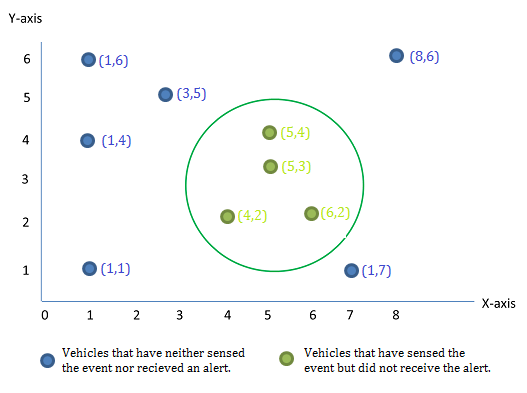
\includegraphics[width=0.5\textwidth]{figs/simulated.png}
    \caption{Mercury event simulation.}
    \label{fig:simulated}
  \end{center}
\end{figure}

%%% Area of Interest overlay
\begin{figure}[ht]
  \begin{center}
    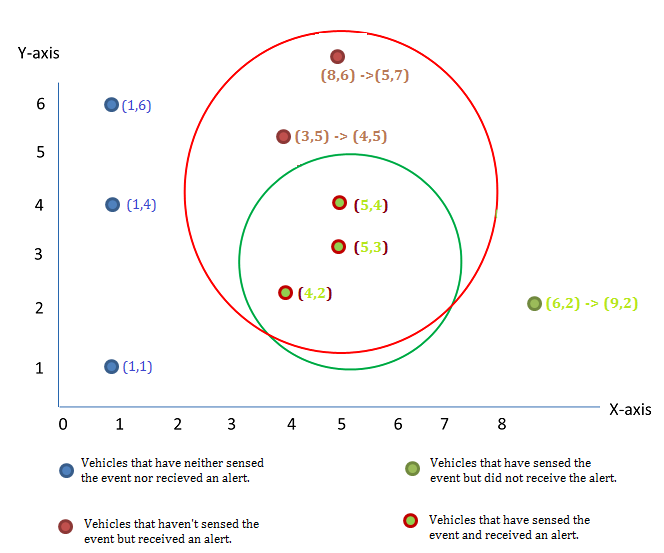
\includegraphics[width=0.5\textwidth]{figs/aoi.png}
    \caption{Mercury Area Of Interest.}
    \label{fig:aoi}
  \end{center}
\end{figure}

By the time AOI message from Message Broker has reached the vehicles
we have observed the vehicle which has sensed the event at location
(6,2) has moved away from the region. This vehicle didn’t receive any
alert from Mercury.  There were two other vehicles that are at
location (3,5) and (8,6) and have moved into the AOI calculated by
Message Broker both these vehicles received the message. And the three
of four vehicles which have sensed the event were still falling within
the Message Broker’s AOI and have received an alert.
   
Through this experiment we have verified that all the vehicles within the
AOI of Message Broker have received an alert irrespective of sensing
the event and those vehicles which are out of the AOI have not
received the vehicle.

\subsection{Latency Micro-benchmark}

{\bf PUT STUFF HERE.}

\comment{
\begin{itemize}
\item Discuss evaluation approach.
  \begin{itemize}
  \item Do evaluation in PhantomNet using OpenEPC with emulated RAN.
  \item Use vehicle mobility model, SUMO, to drive realistic mobility scenarios.
  \item Use SUMO output (position, primarily), to trigger handover.
  \end{itemize}
\item Types of evaluations to perform.
  \begin{itemize}
  \item Functional: Endpoints connect and are tracked properly (handover).
  \item Functional: Areas of Interest are interpreted properly.
  \item Scaling: Run simulated/emulated scenarios with dozens of endpoints.
  \item Scaling: Increase message/sec load and observe system response times.
  \end{itemize}
\end{itemize}
}
